\section{Numerik}
\subsection{Diskretisierung}
\subsubsection{1.Ableitung}

$$g'(x)\approx \frac{g(x+\Delta x)-g(x)}{\Delta x} \qquad\qquad \text{oder}
\qquad\qquad \boxed{g'(x)\approx \frac{g(x+\Delta x)-g(x-\Delta x)}{2\Delta
x}}\qquad \text{(Zentrale Differenz: Bessere Qualität)}$$
\subsubsection{2.Ableitung}
$\boxed{g''(x)\approx \frac{g(x-\Delta x)-2 g(x) + g(x+ \Delta x)}{\Delta x^2}}$ ist für zweite (bessere Qualität) Version die Gleiche

\subsection{FDM}
\textbf{TIPP:} Bei Anfangsbedingungen ungleich Null das Gleichungssystem selber von Hand herleiten, reduziert die Chance auf Fehler.
\subsubsection{Grundgleichung: $-u''(x)=f(x)$}
$ A^{(n)} \tilde{u}^{(n)} =f^{(n)}   $\\
$A^{(n)}= \frac{1}{\Delta x^2} \tridiag_{n-1} (-1,2,-1) = \frac{1}{\Delta x^2}
  \begin{bmatrix}
             2& -1 & 0 & \ldots \\
             -1& 2 & -1 & \ldots \\
              0& -1 & 2 & \ldots \\
              0& 0 & -1 & \ldots \\
             \ldots 
           \end{bmatrix}$\qquad (eine $(n-1)\times(n-1)$-Matrize)\\ 
Randwert: $\tilde{u}(0)= a; \tilde{u}(n)=b $;
$A^{(n)}=\tilde{u}^{(n)} =\begin{bmatrix}
             f(0) + \tilde{u}(0) \\
             f(1) \\
             \vdots  \\
             f(n) + \tilde{u}(n)
           \end{bmatrix} $\\
\subsubsection{Grundgleichung: $T''(x) -  h T(x) = T_A$}
$-T'' + h T(x) = h T_A$\\
$A^{(n)}= \frac{1}{\Delta x^2} \tridiag_{n-1}
(-1,2+h\Delta x^2,-1) = \frac{1}{\Delta x^2}
  \begin{bmatrix}
             2+h\Delta x^2& -1 & 0 & \ldots \\
             -1& 2+h\Delta x^2 & -1 & \ldots \\
              0& -1 & 2+h\Delta x^2 & \ldots \\
              0& 0 & -1 & \ldots \\
             \ldots 
           \end{bmatrix} $\\    
              
\subsubsection{Beispiel Hausübung 7}
Gegeben: $ u''(x)=4(u(x)-x) $ mit den Randwerten $ u(0)=0 $  und $ u(1)=2 $ mit $\Delta x=1/3$.
\\
Gesucht: $ \tilde{u}(\frac{1}{3}) $ und $ \tilde{u}(\frac{2}{3}) $
\\
Lösen: Die Ableitung von $ u'' $ einsetzen, siehe oben, ergibt die allgemeine Gleichung von $ \frac{u(x-\Delta x)-2 u(x) + u(x+ \Delta x)}{\Delta x^2} =4 (u(x)-x) $, für die Punkte P1 und P2 ergibt das.
\\
P1: $ \frac{0-2 \tilde{u}(\frac{1}{3}) + \tilde{u}(\frac{2}{3})}{(\frac{1}{3})^2} =4(\tilde{u}(\frac{1}{3})-\frac{1}{3}) $
\qquad \qquad
P2: $ \frac{\tilde{u}_1(\frac{1}{3})-2 \tilde{u}(\frac{2}{3}) + 2}{(\frac{1}{3})^2} =4(\tilde{u}(\frac{2}{3})-\frac{2}{3}) $
\\
Nun das Gleichungssysteme lösen ergibt $ \tilde{u}(\frac{1}{3}) $ und $ \tilde{u}_2(\frac{2}{3}) $          
           
           
\subsection{Konvergenz}
Ein Modell ist konvergent wenn bei $n\rightarrow\infty$ die Schätzung $\tilde{u}$ und $u$ übereinstimmt.\\

$\boxed{||v||_{\Delta x}=\sqrt{\Delta x (v_1^2+v_2^2 + \ldots v_{n-1}^2)}= \sqrt{\Delta
x}||v||}$\\
Es konvergiert wenn: $\lim\limits_{n\to \infty
}||\tilde{u}^{(n)}-u^{(n)}||=0=\sqrt{\frac{1}{n}}||\tilde{u}^{(n)}-u^{(n)}=\sqrt{\frac{1}{n}}\sqrt{(\tilde{u}_1)-u_1)^2
+ \ldots + \tilde{u}_{n-1}-u_{n-1}}$\\

\subsection{Konsistenz}
Ein Modell ist konsistent wenn das Modell durch Vereinfachung mit der Realität übereinstimmt.

Globaler Konsistenzfehler (Residuum): $\boxed{||r^{(n)}||_{1/n}\leq \frac 1{12}\max\limits_{\xi\in[0,1]}|f''(\xi)|\cdot \Delta x^2}$

\subsubsection{Residuum}
Exakt: $A^{(n)}\cdot \tilde{u}^{(n)}-f^{(n)}=0$\\
Residuum: $A^{(n)}\cdot (u^{(n)}-\tilde{u}^{(n)})=r^{(n)}$

Eine Approximationsverfahren ist Konsistent, wenn $\boxed{\lim\limits_{n\rightarrow \infty}||r^{(n)}||_{1/n}=0}$ gilt.\\

Konsistenz ist eine notwendige, aber nicht hinreichende Bedingung für die Konvergenz eines Verfahrens.

\subsubsection{Taylor}
$g(x)= \sum\limits_{k=0}^n\frac{1}{k!} g^{(n)}(x_0)(x-x_0)^k +
\frac{1}{(n+1)!}g^{(n+1)}(\xi)(x-x_0)^{n+1}$ = Taylor
Approximationspolynom  + Lagrangsches Restglied ($\xi$ ist unabhängig von $x,x_0$)\\

Alternative
$ f(x_0+h)=f(x_0)+f'(x_0)\frac{h}{1!}+...+f^{(n)}(x_0)\frac{h^n}{n!}+R_n(h) $ wobei $ h = x - x_0 $




\subsubsection{Vorwärt/Rückwärtsdifferenz}
$g'(x) - \frac{g(x+\Delta x) + g(x)}{\Delta x}= O(\Delta x) = 
\frac{g''(\xi_1)}{2}\Delta x^2 \Rightarrow$  1. Ordnung


\subsubsection{Zentraldifferenz}
$g'(x) - \frac{g(x+\Delta x) + g(x-\Delta x)}{2\Delta x}= O(\Delta x^2) = 
\frac{g''(\xi_1)}{2}\Delta x^2 \Rightarrow$ 2. Ordnung



\subsubsection{2.Ableitung}
$g''(x) - \frac{g(x+\Delta x) -2 g(x)+ g(x-\Delta x)}{2\Delta x}= O(\Delta x^2)
= \frac{g''(\xi_1)}{2}\Delta x^2 \Rightarrow$ 1. Ordnung

\subsection{Stabilität}
Die Stabilität einer Matrize kann über deren Norm $||A||_*$ bestimmt werden.\\

Es gilt: $||A||_*=\max\limits_{||X||_*=1}||A\cdot x||_*$\qquad$||A\cdot x||_*\leq||A||~||x||_*$\\

Ein Approximationsverfahren ist stabil wenn, wenn unabhängig von der konstante $C$ gilt:
$\boxed{||{A^{(n)}}^{-1}||\leq C}$\\



Die Bestimmung von $||A||$ ist im Allgemeinen nicht einfach, darum wird $||A||$ oft über den Umweg der Diagonalisierung von A bestimmt.

$y=A\cdot x\qquad\Rightarrow\qquad\tilde{y}=D\cdot\tilde{x}$\qquad mit\qquad $D=\begin{bmatrix}\lambda_1&&\\&\ddots&\\&&\lambda_n\end{bmatrix}$\\

Es gilt $TAT^T=D$, wobei T die Transformationsmatrix vom $x$-Koordinatensystem zum $\tilde{x}$-Koordinatensystem darstellt. $T$ ist orthogonal.
Die Diagonalelemente $\lambda_1,\ldots,\lambda_n$ werden auch Eigenwerte genannt.\\

Eine Approximationsformel ist stabil wenn: $\boxed{||A||=\max\limits_{k}|y_k|\leq C}$\\

Eigenwerte bestimmen: $\boxed{\det(A-\lambda I)=|A-\lambda I|=0}\qquad \Rightarrow \qquad \lambda_1,\ldots,\lambda_n$\\
Eigenvektoren bestimmen (für jedes $\lambda_i$): $A-\lambda_i I=0\qquad \Rightarrow \qquad v_1,\ldots,v_n$\\

\subsection{FDM für elliptisch PDGL (Poisson: $\Delta u = f$)}
%Dirichletsche Randbedingung ($u(x,y)= f(x,y) \forall (x,y)\epsilon \delta G)$\\

Gleichung:    $-\Delta u(x,y)= f(x,y) $
$\frac{g(x+\Delta x,y ) -2 g(x,y)+ g(x-\Delta x,y)}{2\Delta x} +
\frac{g(x,y+\Delta y) -2 g(x,y)+ g(x,y-\Delta y)}{2\Delta y}$\\

$h=\Delta x = \Delta y \Rightarrow \boxed{\frac 1 {h^2} (\tilde{u}_{j,k+1} +
\tilde{u}_{j+1,k} + \tilde{u}_{j,k-1} + \tilde{u}_{j-1,k} - 4 \tilde{u}_{j,k})
= f_{j, k}}$\\[0.4cm]


$B \tilde{u} = f \Rightarrow B= \begin{bmatrix}
             T& D & 0 & \ldots \\
             D& T & D & \ldots \\
              0& D & T & \ldots \\
              0& 0 & D & \ldots \\
             \ldots 
           \end{bmatrix}$
wobei $T=\begin{bmatrix}
             4& -1 & 0 & \ldots \\
             -1& 4 & -1 & \ldots \\
              0& -1 & 4 & \ldots \\
              0& 0 & -1 & \ldots \\
             \ldots 
           \end{bmatrix}$
und $D=\begin{bmatrix}
             -1& 0& 0 & \ldots \\
             0 & -1 &  & \ldots \\
              0& 0&-1 & \ldots \\
             \ldots 
           \end{bmatrix}$

           
\subsubsection{Irreguläre Gitter (für den Rand)}
\begin{minipage}{5cm}
	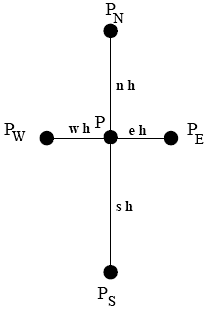
\includegraphics[width=5cm]{Content/Numerik/irregulaereGitter.png}

\end{minipage}
\hfill
\begin{minipage}{14cm}

\begin{multline*}
\bigg(\frac{u(x+eh,y)-u(x,y)}{e(e+w)} +\frac{u(x+wh,y)-u(x,y)}{w(e+w)}+\frac{u(x+nh,y)-u(x,y)}{n(n+s)}\\ +\frac{u(x+sh,y)-u(x,y)}{n(n+s)}\bigg)\frac{2}{h^2}
=f(x,y)
\end{multline*}
oder
\begin{multline*}\frac{u(P_E) - u(P)}{e(e+w)} + \frac{u(P_W) - u(P)}{w(e+w)} + \frac{u(P_N) - u(P)}{n(n+s)} + \frac{u(P_S) - u(P)}{s(n+s)} = \frac{h^2}{2} f(x,y)
\end{multline*}

Wenn $\Delta x, \Delta y$ konstant ($wh = eh,\, nh = sh$) sowie $h=1$:
$$
\frac{u_E + u_W - 2 u_P}{\Delta x^2} + \frac{u_N + u_S - 2 u_p}{\Delta y^2} = f(x,y)
$$
\end{minipage}
\subsubsection{Neumann Rand 
%$\partial_n u(x,y) \forall (x,y) \epsilon \partial_n G$
}
\begin{minipage}{6cm}
	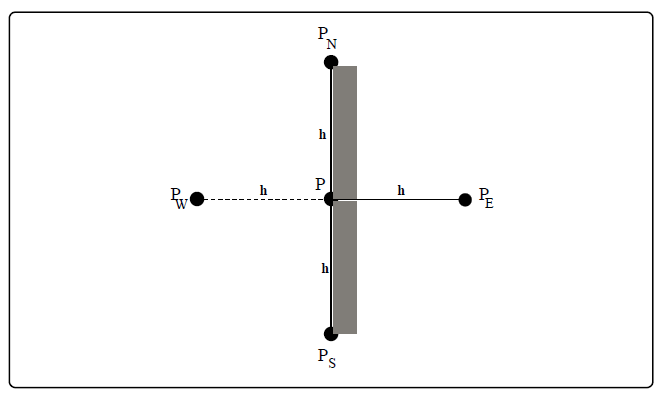
\includegraphics[width=6cm]{Content/Numerik/NeumannRand.png}


\end{minipage}
\hfill
\begin{minipage}{13cm}
In einem Randpunkt P liegen wie in der Abbildung ersichtlich, $P_N$ und $P_S$ auf dem Rand von Omega, $P_W$ liegt ausserhalb von Omega.\\
In P sei die Neumannsche Randbedingung: $\boxed{\partFrac{u}{n}(P)=g(P)}$\\
$u_x(P)=\frac{u(P_E)-u(P_W)}{2h}\quad\Rightarrow\quad u(P_W)=u(P_E)-2h\cdot u_x(P)$\\

$\boxed{\frac{2u(P_E) + u(P_N) +
u(P_S)- 4 u(P) - 2h\cdot u_x(P)}{h^2}}$\\


\textbf{Spiegelmethode}:\\
Wenn $u_x(x,y) = 0$, dann spricht man auch von der Spiegelmethode. Die Punkte $P_W$ und $P_E$ weisen dann die gleiche Wertigkeit auf ($P_W=P_E$).
\end{minipage}


\subsection{FDM für parabolische PDGL}
	Wärmeleitungsgleichung: $\boxed{u_t(x,t)=u_{xx}(x,t)}$\qquad $f(0)=f(1)=0$ \qquad$ \overset{\_}{\Omega}=[0,1]\times [0,\infty]$\\
	
	Randbedingungen: $u(x,0)=f(x) \qquad u(0,t)=u(1,t)=0\qquad x\in(0,1) \qquad t\in[0,\infty)$
\subsubsection{Explizites Verfahren (Richardson-Verfahren)}
$\boxed{\frac{\tilde{u}(x,t+\Delta t) - \tilde{u}(x,t)}{\Delta t} = 
\frac{\tilde{u}(x+\Delta x, t)-2\tilde{u}(x,y) + \tilde{u}( x - \Delta x, t )} {\Delta x^2}} \qquad \Delta x=\frac{x_{max}-x_{min}}{n}\qquad \Delta t=\frac r{n^2} \qquad \boxed{r=\frac{\Delta
t}{\Delta x^2}}$\\

\textbf{Idee:} Aus den Positionen $k$ wird $k+1$ berechnet: $\tilde{u}_{j,k+1} = r \tilde{u}_{j-1,k} + (1-2r)\tilde{u}_{j,k} + r \tilde{u}_{j+1,k}$\\
Diskretisierung von t: k, k+1, \ldots\\
Diskretisierung von x: j, j+1, \ldots\\

\begin{itemize}
\item Initialisierung, Randbedingung: $\tilde{u}_{j,0}=f(j/n)$ \qquad $\tilde{u}_{0,k}=\tilde{u}_{n,k}=0$
\item Approximationsmatrize: $C^{(n)}=\tridiag_{n-1}(r,1-2r,r)=\begin{bmatrix}
1-2r& r		& 0		& 0 	&\cdots\\
r	& 1-2r  & r		& 0		&\cdots\\
0	& r		& 1-2r 	& r 	&\cdots\\
0	& 0		& r		& 1-2r 	&\cdots\\
\vdots&	\vdots&\vdots&\vdots&\ddots	
\end{bmatrix}$ 
\item Einen Schritt berechnen: $\tilde{u}^{(k+1)}=C^{(n)} \tilde{u}^{(k)}$
\item $k$-Schritte berechnen: $\tilde{u}^{(k)}=\big\{C^{(n)}\big\}^k \tilde{u}^{(0)}$
\end{itemize}

\textbf{Konvergenzverhalten:} \\

\begin{minipage}{6cm}
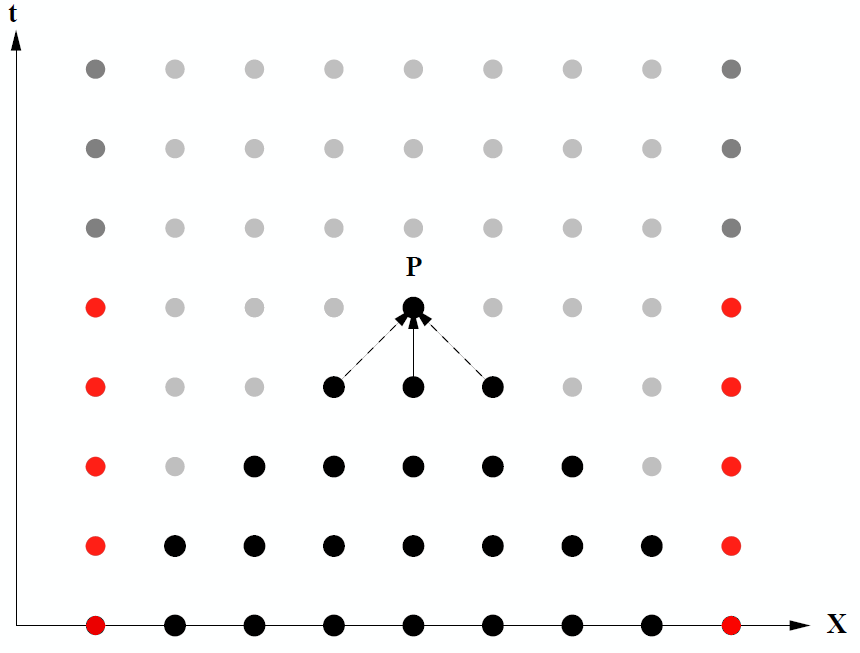
\includegraphics[width=6cm]{Content/Numerik/KonvExplizit.png}
\end{minipage}
\hfill
\begin{minipage}{12cm}
Verfahren ist stabil wenn: $||A^{-1}|| < 1 \qquad \Rightarrow\qquad r < \frac{1}{2}$\\

Dies macht es nötig, die Zeitschritte extrem klein zu wählen. Darum ist das Verfahren auch nicht wirklich praxistauglich, weil sehr hohe Rechenkapazität nötig sind.\\

Der Grund für das schlechte Konvergenzverhalten kann geometrisch visualisiert werden. In die Berechnung des Wertes im Knoten $P$, werden die Werte aller schwarz eingefärbter Knoten eingehen. Von den Randwerten wird nur die 0-te Stufe berücksichtigt.
\end{minipage}
Damit das Verfahren mit $C^k$ für k-Schritte berechnet werden kann, müssen die
rot eingefärbten Werte (links und rechts) gleich 0 sein (Boundary Condition).
Für den Randvektor $\tilde{u}^{(0)}$ werden nur die untersten schwarzen 7 Punkte
eingefüllt.

\subsubsection{Implizites Verfahren}
Im Unterschied zum expliziten Verfahren, das Werte vom vorherigen Zeitpunkt nutzt, wird hier das ein Gleichungssystem global gelöst.\\

$\boxed{\frac{\tilde{u}(x,t) - \tilde{u}(x,t -\Delta t)}{\Delta t} = 
\frac{\tilde{u}(x+\Delta x, t)-2\tilde{u}(x,y) + \tilde{u}( x - \Delta x, t )} {\Delta x^2}}
 \qquad \Delta x=\frac{x_{max}-x_{min}}{n}\qquad \Delta t=\frac r{n^2} \qquad \boxed{r=\frac{\Delta
t}{\Delta x^2}}$\\

$ \tilde{u}_{j,k} = r \tilde{u}_{j-1,k+1} + (1+2r)\tilde{u}_{j,k+1} + r \tilde{u}_{j+1,k+1}$

\textbf{Idee:} Die Ableitungen werden mittels Rückwärtsdifferenz berechnet\\


\begin{itemize}
\item Initialisierung, Randbedingung: $\tilde{u}_{j,0}=f(j/n)$ \qquad $\tilde{u}_{0,k}=\tilde{u}_{n,k}=0$
\item Approximationsmatrize: $E^{(n)}=\tridiag_{n-1}(-r,1+2r,-r)=\begin{bmatrix}
1+2r& -r		& 0		& 0 	&\cdots\\
-r	& 1+2r  & -r		& 0		&\cdots\\
0	& -r		& 1+2r 	& -r 	&\cdots\\
0	& 0		& -r		& 1+2r 	&\cdots\\
\vdots&	\vdots&\vdots&\vdots&\ddots	
\end{bmatrix}$ 
\item Einen Schritt berechnen: $\tilde{u}^{(k+1)}=\left\{E^{(n)}\right\}^{-1} \tilde{u}^{(k)}$
\item $k$-Schritte berechnen: $\tilde{u}^{(k)}=\left\{E^{(n)}\right\}^{\bm{-}k} \tilde{u}^{(0)}$
\end{itemize}

\textbf{Vorteil:} Das implizite Verfahren ist immer stabil, unabhängig von der Zeitauflösung $\Delta t$\\
\textbf{Nachteil:} Aufwendige Matrixinversion nötig.

\subsubsection{Crank Nicolson -Verfahren (gemischtes Verfahren)}

Die Idee des Verfahrens von Crank-Nicolson ist es die beiden Approximationen

$\boxed{\frac{\tilde{u}(x,t+\Delta t) - \tilde{u}(x,t)}{\Delta t} = 
\frac{\tilde{u}(x+\Delta x, t)-2\tilde{u}(x,y) + \tilde{u}( x - \Delta x, t )} {\Delta x^2}}$
$\boxed{\frac{\tilde{u}(x,t) - \tilde{u}(x,t -\Delta t)}{\Delta t} = 
\frac{\tilde{u}(x+\Delta x, t)-2\tilde{u}(x,y) + \tilde{u}( x - \Delta x, t )} {\Delta x^2}}$

zu mitteln. Mit dieser Idee geht das stetige Problem in folgendes diskretes Problem über:

$-r \tilde{u}_{j-1,k+1} + (2+2r)\tilde{u}_{j,k+1} - r \tilde{u}_{j+1,k+1} = r
\tilde{u}_{j-1,k+1} + (2-2r)\tilde{u}_{j,k+1} + r \tilde{u}_{j+1,k+1} $

Wie bei den anderen Verfahren gilt: $\Delta x=\frac{x_{max}-x_{min}}{n}\qquad \Delta t=\frac r{n^2} \qquad \boxed{r=\frac{\Delta
t}{\Delta x^2}}$
\begin{itemize}
\item Initialisierung, Randbedingung: $\tilde{u}_{j,0}=f(j/n)$ \qquad $\tilde{u}_{0,k}=\tilde{u}_{n,k}=0$
\item Approximationsmatrizen:\\
$F^{(n)}=E^{(n)}+I=\tridiag_{n-1}(-r,2+2r,-r)=\begin{bmatrix}
2+2r& -r	& 0		& 0 	&\cdots\\
-r	& 2+2r  & -r	& 0		&\cdots\\
0	& -r	& 2+2r 	& -r 	&\cdots\\
0	& 0		& -r	& 2+2r 	&\cdots\\
\vdots&	\vdots&\vdots&\vdots&\ddots	
\end{bmatrix}$\\
$G^{(n)}=C^{(n)}+I=\tridiag_{n-1}(~r,~2-2r,~r~)=\begin{bmatrix}
2-2r& r		& 0		& 0 	&\cdots\\
r	& 2-2r  & r		& 0		&\cdots\\
0	& r		& 2-2r 	& r 	&\cdots\\
0	& 0		& r		& 2-2r 	&\cdots\\
\vdots&	\vdots&\vdots&\vdots&\ddots	
\end{bmatrix}$ 
\item Einen Schritt berechnen: $\tilde{u}^{(k+1)}=\left\{F^{(n)}\right\}^{-1} \cdot G^{(n)}\cdot \tilde{u}^{(k)}$
\item $k$-Schritte berechnen: $\tilde{u}^{(k)}=\left(\left\{F^{(n)}\right\}^{-1} \cdot G^{(n)}\right)^{k}\cdot \tilde{u}^{(0)}$
\end{itemize}

\subsection{(FDM für Hyperbolische PDGL)}

$$u_{tt}=u_{xx} = \text{homogen}$$
$$u_{tt} -u_{xx}= v(x,t) = \text{inhomogen}$$

$$\Longrightarrow u_{j,k+1}=r^2 u_{j-1,k} + 2(1-r^2)u_{j,k}+ r^2
u_{j+1,k}-u_{j,k-1} \quad \text{(Leap-Frog-Schema)}$$
\subsubsection{Anfangsbedingungen}
$$\tilde{u}_{j,0} = f(j\Delta x); u_{j,1}= f(j\Delta x) + g(j\Delta x)\Delta t$$
(f(x)= Anfangsfunktion; g(x)=Ableitung; $r = \frac{\Delta t}{\Delta x}$)

\subsubsection{Transportgleichung}
$$u_x(x,t) + u_t(x, t) = 0; u(x,0)=P(x-t)$$
$$\frac{u(x,t+\Delta t)-u(x,t)}{\Delta t} = \frac{u(x,t) - u(x-\Delta x,
t)}{\Delta x}$$

\subsection{FVM (Finite Volumen Methode, Verfahren von Voronoi)}
$\Delta u=0$\qquad in \quad$\Omega$\\
$u(x,y)=f(x,y)$ \qquad auf \quad$\partial\Omega$\\
Der Satz von Gauss sagt: $\boxed{\oint\limits_{\Gamma}{\Delta u(x,y) dx dy}=\int\limits_{\Gamma}{\mathrm{div}~\mathrm{grad}~ u(x,y) dx dy}=\oint\limits_{\partial\Gamma}{\mathrm{grad}~ u(x,y) d\vec{n}}}$\\


Wobei der Randnormalvektor $\vec{n}$ immer senkrecht gegen das Aussengebiet $\Gamma$ gerichtet wird.\\

$\Rightarrow$ $\oint\limits_{\Gamma}{\Delta u(x,y) dx dy}=\oint\limits_{\partial\Gamma}{\mathrm{grad}~ u(x,y) d\vec{n}}=0$

\begin{minipage}{4cm}
	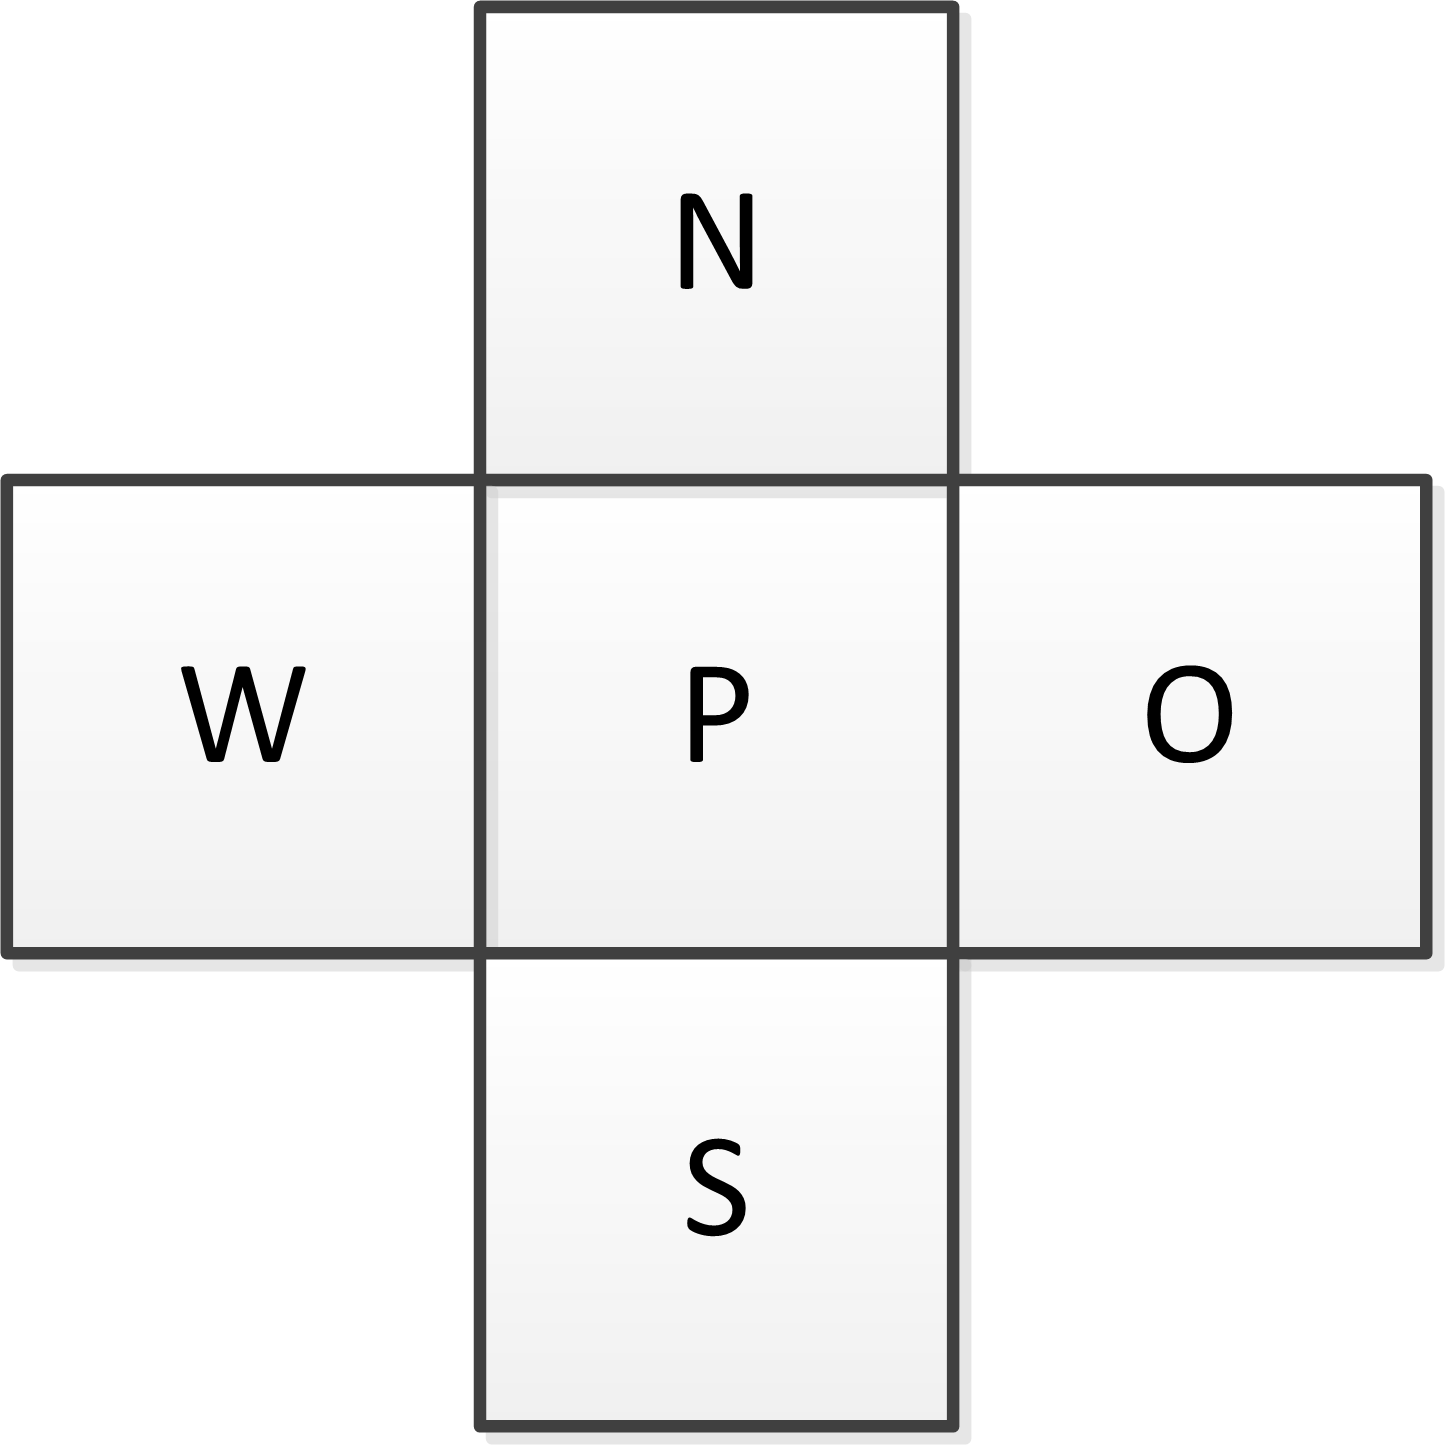
\includegraphics[width=4cm]{Content/Numerik/FVMPrinzip.png}
\end{minipage}
\hfill
\begin{minipage}{14cm}
	$\frac{u(P_E)-u(P_P)}{h}\cdot h+\frac{u(P_N)-u(P_P)}{h}\cdot h+\frac{u(P_W)-u(P_P)}{h}\cdot h+\frac{u(P_S)-u(P_P)}{h}\cdot h\approx 0$\\
	
	$\Rightarrow\tilde{u}(P_E)+\tilde{u}(P_N)+\tilde{u}(P_W)+\tilde{u}(P_S)-4\cdot\tilde{u}(P_P)=0$
\end{minipage}

\textbf{Vorteile:}\\
\begin{itemize}
\item Man kann mit Flussgrössen und Bilanzen rechnen, dadurch kann der
Laplace-Operator $(\Delta)$ verzichtet werden und somit die aufwendige Mathematik umgangen werden.
\item Es kann mit komplizierten Geometrien gerechnet werden.  
\end{itemize}

\begin{minipage}{6cm}
	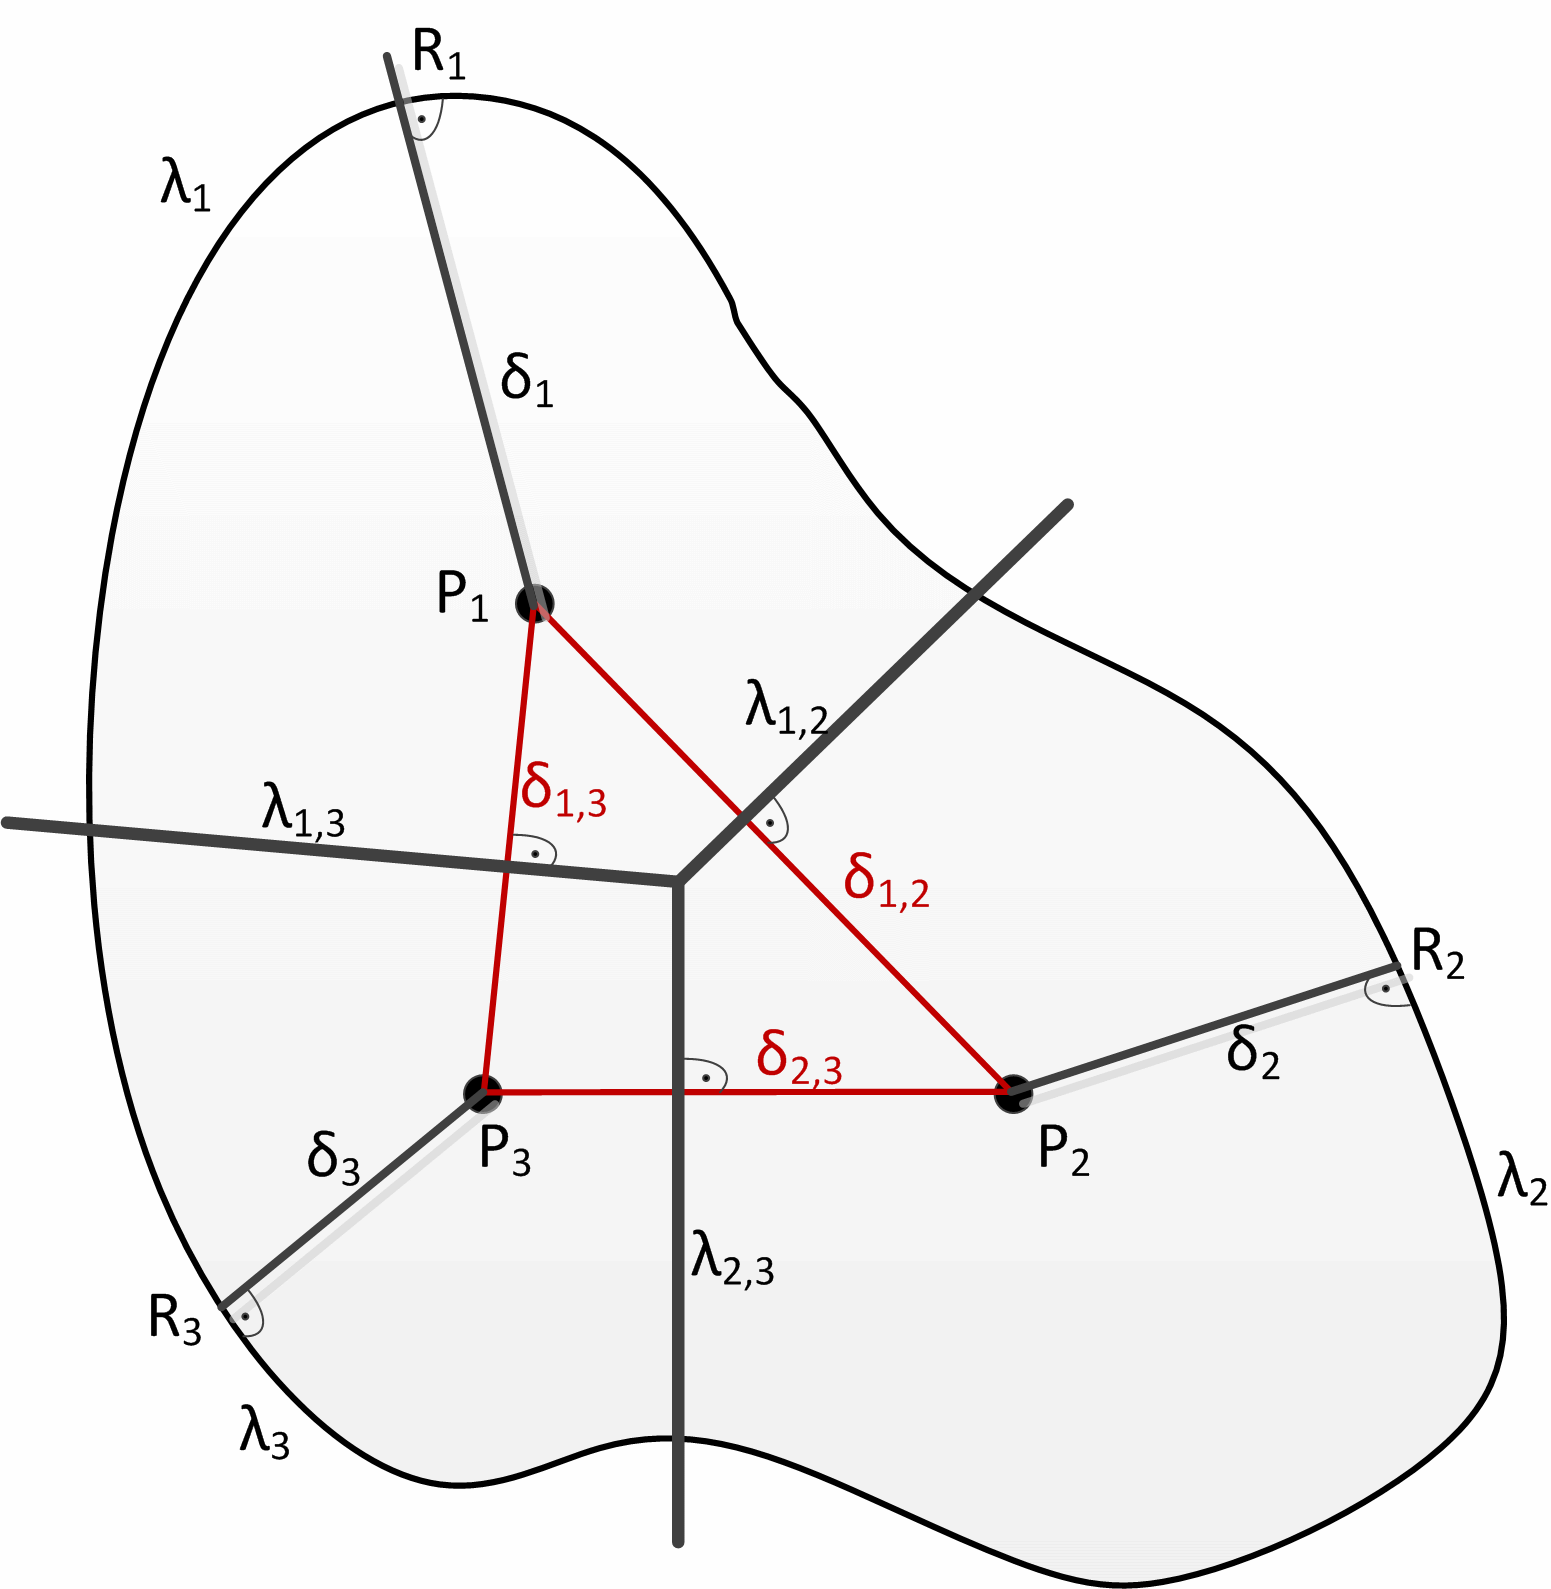
\includegraphics[width=6cm]{Content/Numerik/FVM1.png}
\end{minipage}
\hfill
\begin{minipage}{12cm}
\textbf{Vorgehen bei der Berechnung:}\\
\begin{enumerate}
\item Punkte $P_1,\ldots,P_n$ wählen.
\item Aufteilen des Bereichs in kleine Teilbereiche, z.B. durch Mittelsenkrechte
\item Rand diskretisieren.\\
\end{enumerate}

Für P1-Zelle:\quad $\frac{\tilde{u}(P_2)-\tilde{u}(P_1)}{\delta_{1,2}}\cdot\lambda_{1,2}+\frac{\tilde{u}(P_3)-\tilde{u}(P_1)}{\delta_{1,3}}\cdot\lambda_{1,3}+\frac{\tilde{u}(R_1)-\tilde{u}(P_1)}{\delta_1}\cdot\lambda_1=0$\\

Für P2-Zelle:\quad $\frac{\tilde{u}(P_1)-\tilde{u}(P_2)}{\delta_{1,2}}\cdot\lambda_{1,2}+\frac{\tilde{u}(P_3)-\tilde{u}(P_2)}{\delta_{2,3}}\cdot\lambda_{2,3}+\frac{\tilde{u}(R_2)-\tilde{u}(P_2)}{\delta_2}\cdot\lambda_2=0$\\

Für P3-Zelle:\quad $\frac{\tilde{u}(P_2)-\tilde{u}(P_3)}{\delta_{2,3}}\cdot\lambda_{2,3}+\frac{\tilde{u}(P_1)-\tilde{u}(P_3)}{\delta_{1,3}}\cdot\lambda_{1,3}+\frac{\tilde{u}(R_3)-\tilde{u}(P_3)}{\delta_3}\cdot\lambda_3=0$\\
\end{minipage}

\begin{minipage}{6cm}
	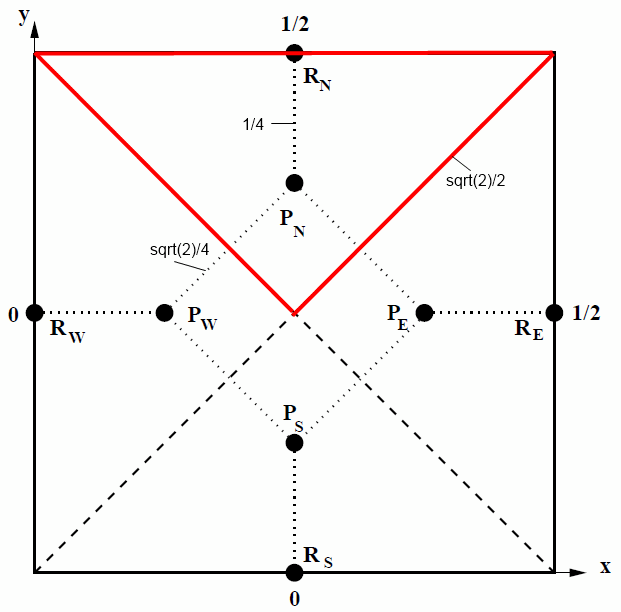
\includegraphics[width=6cm]{Content/Numerik/FVM2.png}
\end{minipage}
\hfill
\begin{minipage}{12cm}

 $\frac{\tilde{u}(P_E)-\tilde{u}(P_N)}{1/4\cdot\sqrt{2}}\cdot\frac{\sqrt{2}}{2}+\frac{\tilde{u}(P_W)-\tilde{u}(P_N)}{1/4\cdot\sqrt{2}}\cdot\frac{\sqrt{2}}{2}+\frac{\tilde{u}(R_N)-\tilde{u}(P_N)}{1/4}\cdot 1=0$\\
 
 $(\tilde{u}_E-\tilde{u}_N)\cdot 2 + (\tilde{u}_W-\tilde{u}_N)\cdot 2 + (1/2-\tilde{u}_N)\cdot 4=0$\\
 
 $0\cdot\tilde{u}_S+2\cdot\tilde{u}_E+2\cdot\tilde{u}_W-8\cdot\tilde{u}_N+2=0$
 

\end{minipage}

\begin{minipage}{6cm}
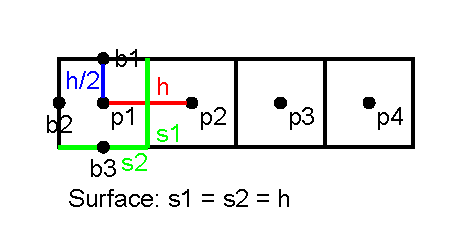
\includegraphics[width=6cm]{Content/Numerik/fvm_beispiel.pdf}
\end{minipage}
\hfill
\begin{minipage}{12cm}

u1: $\frac{u(b_1) - u(p_1)}{h/2} \cdot h + \frac{u(b_2) - u(p_1)}{h/2} \cdot h +
\frac{u(b_3) - u(p_1)}{h/2} \cdot s_2 + \frac{u(p_2) - u(p_1)}{h} \cdot s_1 $\\
\colorbox{yellow}{Achtung wenns schnell gehen muss: $\frac{u(b_2) - u(p_1)}{h/2}
\cdot h = (u(b_2) - u(p_1)) \cdot 2$}

\end{minipage}

\clearpage
\section{FEM}

Der Vektorraum $\mathbb{V}$ hat undendlich viele Dimensionen. Falls wir n unabhängige Funktionen $v_1,\ldots,v_n$ wählen, dann spannen die Funktionen $a_1\cdot v_1(x)+\ldots+a_n\cdot v_n(x)$ einen n dimensionalen Teilraum $\mathbb{V}^{(n)}$  von $\mathbb{V}$ auf. Dabei gilt:\\

$\boxed{\tilde{u}^{(n)}=a_1\cdot v_1(x)+\ldots+a_n\cdot v_n(x)}$
\subsection{Das Verfahren von Ritz}
\textbf{Ritzsche Matrize: }
$R^{(n)}=\begin{bmatrix}
	R_{1,1}& R_{1,2}&\cdots\\
	R_{2,1}& R_{2,2}&\cdots\\
	\vdots & \vdots &\ddots\\
\end{bmatrix}$ \qquad mit \qquad $R_{j,k}^{(n)}=\int\limits_{0}^{1}{v_j'(x)\cdot
v_k'(x) dx}$\\
\textbf{Ritzscher Vektor: } 
$r^{(n)}=\begin{bmatrix}
	r_1\\
	r_2\\
	\vdots\\
\end{bmatrix}$ \qquad mit \qquad $r_{k}^{(n)}=\int\limits_{0}^{1}{f(x)\cdot v_k(x) dx}$\\

\textbf{Lösung nach Ritz:} $R^{(n)}\cdot a=r^{(n)}\qquad \Rightarrow \qquad a=\left\{R^{(n)}\right\}^{-1}\cdot r^{(n)}$
\subsection{Das Verfahren von Galerkin}
\textbf{Galerksche Matrize: }
$G^{(n)}=\begin{bmatrix}
	G_{1,1}& G_{1,2}&\cdots\\
	G_{2,1}& G_{2,2}&\cdots\\
	\vdots & \vdots &\ddots\\
\end{bmatrix}$ \qquad mit \qquad $G_{j,k}^{(n)}=\int\limits_{0}^{1}{\underbrace{(v_j''(x))}_{v_j \text{ in Form von DGL!}}\cdot v_k(x) dx}$\\
\textbf{Galerkscher Vektor: } 
$g^{(n)}=\begin{bmatrix}
	g_1\\
	g_2\\
	\vdots\\
\end{bmatrix}$ \qquad mit \qquad $g_{k}^{(n)}=\int\limits_{0}^{1}{f(x)\cdot v_k(x) dx}$\\

\textbf{Lösung nach Galerkin:} $G^{(n)}\cdot a+g^{(n)}=0\qquad \Rightarrow
\qquad a=\textcolor{red}{\mathbf{-}}\left\{G^{(n)}\right\}^{-1}\cdot g^{(n)}$ \quad nach Ritz $G^{(n)} = -R^{(n)} \quad g^{(n)} = r^{(n)}$\\

Die obige Matrix ist nur für die PDGL $-u''(x) = f(x)$ mit dem Ansatz
$\tilde{u}(x) = a_1 \cdot v_1(x) + a_2 \cdot v_2(x)$ gültig. Ansonsten muss ein
Gleichungssystem für $v_k$ = $v_1$ und $v_2$ aufgestellt werden (Beispiel
für DGL: $u''(x) + u(x) + x = 0$):\\
$\int\limits_{0}^{1}{(a_1 \cdot v_1''(x) + a_2 \cdot v_2''(x) + a_1 \cdot
v_1(x) + a_2 \cdot v_2(x) + x) \cdot v_k(x) dx} = 0 \rightarrow G_{j,k}^{(n)}=\int\limits_{0}^{1}(v_j''(x) + v_j(x))\cdot v_k(x) dx$

\subsection{Gewichtete Residuen}
Gewichtungsfunktionen: $\{w_1(x),\ldots,w_n(x)\}$

\textbf{Matrize (gewichtete Residuen): }
$M^{(n)}=\begin{bmatrix}
	M_{1,1}& M_{1,2}&\cdots\\
	M_{2,1}& M_{2,2}&\cdots\\
	\vdots & \vdots &\ddots\\
\end{bmatrix}$ \qquad mit \qquad $M_{j,k}^{(n)}=\int\limits_{0}^{1}{v_j''(x)\cdot w_k(x) dx}$\\
\textbf{Vektor (gewichtete Residuen): } 
$m^{(n)}=\begin{bmatrix}
	m_1\\
	m_2\\
	\vdots\\
\end{bmatrix}$ \qquad mit \qquad $m_{k}^{(n)}=\int\limits_{0}^{1}{f(x)\cdot w_k(x) dx}$\\

\textbf{Lösung der gewichteten Residuen:} $M^{(n)}\cdot a+m^{(n)}=0\qquad \Rightarrow \qquad a=\textcolor{red}{\mathbf{-}}\left\{M^{(n)}\right\}^{-1}\cdot m^{(n)}$

\subsection{Punktkollokation}
Im Sinne einer Punktkollokation (einzelne Punkte müssen zwischen wahrem Resultat und Approximation übereinstimmen) werden $n$ Stützstellen im Intervall von $[0,1]$ gewählt.\\

$\begin{bmatrix}
	v_1''(x_1)& v_2''(x_1)&\cdots\\
	v_1''(x_2)& v_2''(x_2)&\cdots\\
	\vdots& \vdots&\ddots
\end{bmatrix}\cdot
\begin{bmatrix}
a_1\\
a_2\\
\vdots
\end{bmatrix}
=\begin{bmatrix}
-f(x_1)\\
-f(x_2)\\
\vdots
\end{bmatrix}$\qquad Das Gleichungssystem nach a auflösen\\

Die obige Matrix ist nur für die PDGL $-u''(x) = f(x)$ mit dem Ansatz
$\tilde{u}(x) = a_1 \cdot v_1(x) + a_2 \cdot v_2(x)$ gültig. Ansonsten muss die
DGL mit den Ansatzfunktionen aufgestellt und an beiden Punkten eingesetzt
werden, um $a_1$ und $a_2$ zu bestimmen:\\
DGL: $u''(x) + u(x) = -x$ $\Rightarrow$ Gleichung an Punkt 1: $a_1 \cdot
v_1''(x_1) + a_2 \cdot v_2''(x_1) + a_1 \cdot v(x_1) + a_2 \cdot v(x_1) = - x_1$




\subsection{Bereichskollokation}
Im Gegensatz zur Punktkollokation müssen nicht einzelne Punkte sondern ganze Bereiche (Intervalle $I_k$) übereinstimmen. Für $-u''(x) = f(x)$ wird dieses Gleichungssystem aufgestellt.

$\begin{bmatrix}
	\int_{I_1} v_1'' & \int_{I_1} v_2''& \cdots\\
	\int_{I_2} v_1'' & \int_{I_2} v_2''& \cdots\\
	\vdots& \vdots&\ddots
\end{bmatrix}\cdot
\begin{bmatrix}
a_1\\
a_2\\
\vdots
\end{bmatrix}
=\begin{bmatrix}
-\int_{I_1} f(x)\\
-\int_{I_2} f(x)\\
\vdots
\end{bmatrix}$\qquad Das Gleichungssystem nach a auflösen


\subsection{Das Verfahren von Gauss (MSE)}

\textbf{Gausscher Matrize: }
$Q^{(n)}=\begin{bmatrix}
	Q_{1,1}& Q_{1,2}&\cdots\\
	Q_{2,1}& Q_{2,2}&\cdots\\
	\vdots & \vdots &\ddots\\
\end{bmatrix}$ \qquad mit \qquad $Q_{j,k}^{(n)}=\int\limits_{0}^{1}{v_j''(x)\cdot v_k''(x) dx}$\\
\textbf{Gausscher Vektor: } 
$q^{(n)}=\begin{bmatrix}
	q_1\\
	q_2\\
	\vdots\\
\end{bmatrix}$ \qquad mit \qquad $q_{k}^{(n)}=\int\limits_{0}^{1}{f(x)\cdot v_k''(x) dx}$\\

\textbf{Lösung nach Gauss:} $Q^{(n)}\cdot a+q^{(n)}=0\qquad \Rightarrow \qquad a=\textcolor{red}{\mathbf{-}}\left\{Q^{(n)}\right\}^{-1}\cdot q^{(n)}$

\subsection{Finite Elemente}

Die besprochenen Verfahren setzen die Wahl eines Satzes $v_1(x),\ldots,v_n(x)$ von Grundfunktionen voraus. Bei FEM wird mit lokalen Trägern (Grundfunktionen) gearbeitet, diese sind nur auf einem kleinen Intervall ungleich null. Der Vorteil dieses Vorgehens liegt darin, dass in einem Bereich nur ein Träger die Approximationsfunktion beeinflusst. Der Nachteil liegt in der hohen Anzahl der so benötigten Träger.\\

\textbf{WICHTIG:} Alle Verfahren werden mit einer Diskretisierung von $h=1/3$
vorgestellt.

\subsubsection{Knotenvariablen}
Als erstes werden auf dem Intervall $[0,1]$ $n$, normalerweise gleichverteilte, Knotenstellen eingeführt.

\begin{minipage}{11cm}
Dadurch wird das Intervall $[0,1]$ in Teilintervalle (Maschen) zerlegt.\\
 
Für $n=3$:\quad $I_1=[0,1/3]$\quad $I_1=[1/3,2/3]$\quad $I_1=[2/3,1]$\\

Als nächstes wird jeder Knotenstelle $x_k$ eine Ansatzvariable (Knotenvariable) zugeordnet.\\

Ansatz: \quad $\tilde{u}(0)=a_0$\quad $\tilde{u}(1/3)=a_1$\quad $\tilde{u}(2/3)=a_2$\quad $\tilde{u}(1)=a_3$\\

Zusatzbedingungen:
\begin{tabular}{llll}
$v_0(0)=1$&$v_0(1/3)=0$&$v_0(2/3)=0$&$v_0(1)=0$\\
$v_1(0)=0$&$v_1(1/3)=1$&$v_1(2/3)=0$&$v_1(1)=0$\\
$v_2(0)=0$&$v_2(1/3)=0$&$v_2(2/3)=1$&$v_2(1)=0$\\
$v_3(0)=0$&$v_3(1/3)=0$&$v_3(2/3)=0$&$v_3(1)=1$\\
\end{tabular}
\end{minipage}
\hfill
\begin{minipage}{8cm}
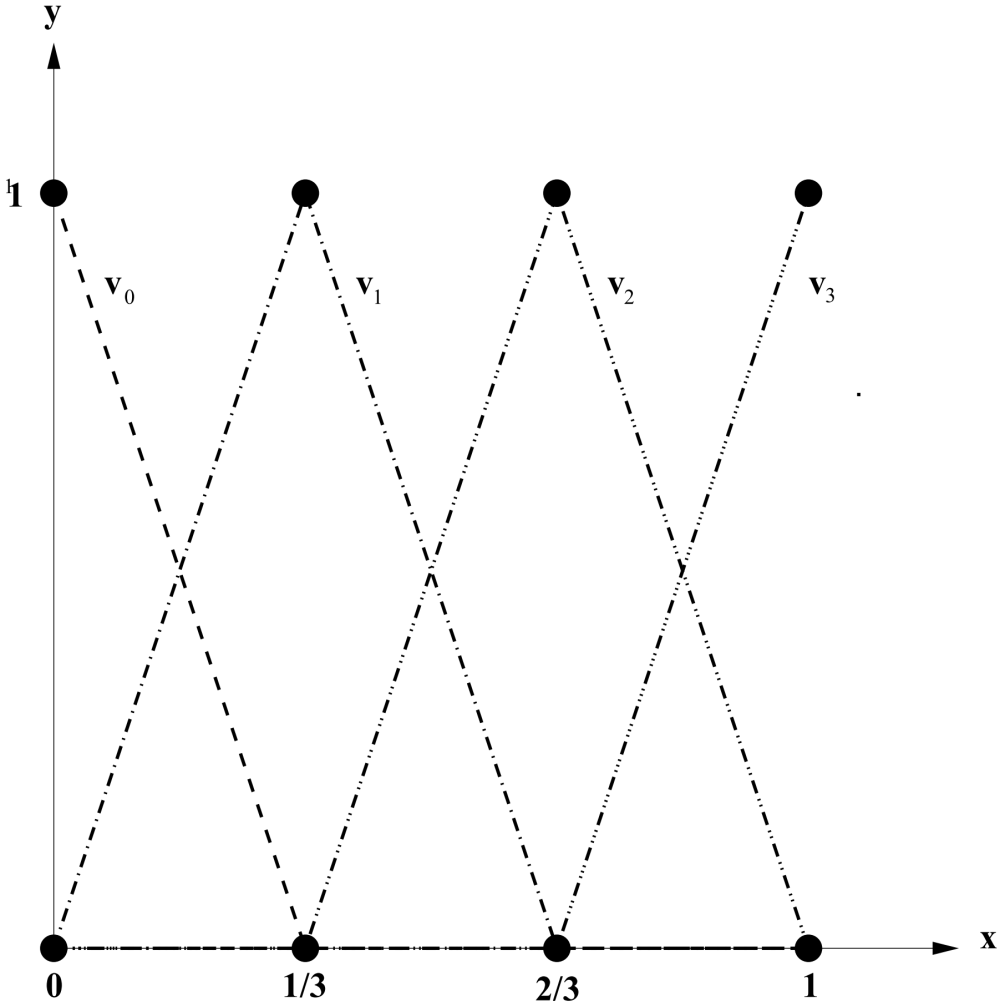
\includegraphics[width=8cm]{Content/Numerik/Traeger1.png}
\end{minipage}


\subsubsection{Formfunktionen}
Die lokalen Grundfunktionen sollen aus Teilstücken einfacher Funktionen, z.B: Polynomen, die nur auf einer einzelnen Masche definiert sind zusammengesetzt werden.\\
Zwei mögliche Formfunktionen sind Beispielsweise:\quad $l_1(x)=1-x$\quad und \quad $l_2(x)=x$\\

\begin{minipage}{8cm}
	\begin{tabular}{lc|c|c}
	$t\in$&$[0,1/3]$&$[1/3,2/3]$&$[2/3,1]$\\
	\hline
	$v_0=$&$1-3x$&$0$&$0$\\
	$v_1=$&$3x$&$2-3x$&$0$\\
	$v_2=$&$0$&$-1+3x$&$3-3x$\\
	$v_3=$&$0$&$0$&$-2+3x$\\
	\end{tabular}
\end{minipage}
\hfill
\begin{minipage}{2cm}
$\Longrightarrow$
\end{minipage}
\hfill
\begin{minipage}{8cm}
	\begin{tabular}{lc|c|c}
	$t\in$&$[0,1/3]$&$[1/3,2/3]$&$[2/3,1]$\\
	\hline
	$v_0=$&$l_1(3x)$&$0$&$0$\\
	$v_1=$&$l_2(3x)$&$l_1(3x-1)$&$0$\\
	$v_2=$&$0$&$l_2(3x-1)$&$l_1(3x-2)$\\
	$v_3=$&$0$&$0$&$l_2(3x-2)$\\
	\end{tabular}
\end{minipage}
\subsubsection{Elementmatrizen}
Grundsätzlich kann die Ansatzvariable durch jedes Verfahren bestimmt werden.
Weil bei einer linearen Ansatzfunktion die zweite Ableitung trivial $(=0)$ ist die Wahl des Ritzschen Verfahren erzwungen.

Die Integrale werden maschenweise ausgewertet:\\

 $\int\limits_{0}^{1}{}=\int\limits_{0}^{1/3}{}+\int\limits_{1/3}^{2/3}{}+\int\limits_{2/3}^{1}{}$\\
 
Durch diesen Ansatz wird die Ritzsche Matrize über jede Masche einzeln berechnet und danach zur globalen Ritzschen Matrize aufsummier:\\

\qquad $R^{(4)}=R^{(4,1)}+R^{(4,2)}+R^{(4,3)}=
\begin{bmatrix}
	* & * & 0 & 0\\
	* & * & 0 & 0\\
	0 & 0 & 0 & 0\\
	0 & 0 & 0 & 0\\
\end{bmatrix}+
\begin{bmatrix}
	0 & 0 & 0 & 0\\
	0 & * & * & 0\\
	0 & * & * & 0\\
	0 & 0 & 0 & 0\\
\end{bmatrix}+
\begin{bmatrix}
	0 & 0 & 0 & 0\\
	0 & 0 & 0 & 0\\
	0 & 0 & * & *\\
	0 & 0 & * & *\\
\end{bmatrix}
$\\

Die mit $*$ bezeichneten $2\times 2$ Matrizen heissen Maschenmatrizen:\\

$M^{(4,1)}=M^{(4,2)}=M^{(4,3)}=
\begin{bmatrix}
	* & *\\
	* & *\\
\end{bmatrix}=3\cdot\begin{bmatrix}
	-1 & 1\\
	1 & -1\\
\end{bmatrix}\qquad\Rightarrow\qquad\boxed{M=\frac 1h\cdot
\underset{\text{\textbf{E}: Elementmatrize}}{\underbrace{\begin{bmatrix}
	-1 & 1\\
	1 & -1\\
\end{bmatrix}}}=\frac 1h\cdot \mathbf{E}}$\\

Die Elementmatrize wird nun in die entsprechende Ritzsche Matrize eingesetzt und überlagert. Für die Quantisierung von $h=1/3$ ergibt sich:\\

$R^{4}=
\begin{bmatrix}
	-3 & 3 & 0 & 0 \\
	3 & -3-3 & 3 & 0 \\
	0 & 3 & -3-3 & 3 \\
	0 & 0 & 3 & -3 \\
\end{bmatrix}=
\begin{bmatrix}
	-3 & 3 & 0 & 0 \\
	3 & -6 & 3 & 0 \\
	0 & 3 & -6 & 3 \\
	0 & 0 & 3 & -3 \\
\end{bmatrix}$\\

Der Ritzsche Vektor muss mittels Integration berechnet werden:\\

$r^4=
\begin{bmatrix}
	\int\limits_{0}^{1}{f(x)\cdot v_0(x)dx}\\
	\int\limits_{0}^{1}{f(x)\cdot v_1(x)dx}\\
	\int\limits_{0}^{1}{f(x)\cdot v_2(x)dx}\\
	\int\limits_{0}^{1}{f(x)\cdot v_3(x)dx}\\
\end{bmatrix}$\\

Das Ritzsche Gleichungssystem dazu ist: $\boxed{R^4\cdot a+r^4=0} \qquad\Rightarrow\qquad a=-\left\{R^4\right\}^{-1}\cdot r^4$\\

\textbf{Anfangsbedingungen:} Die Anfangsbedingungen $a_0$ und $a_n$ können direkt eingesetzt werden.\\

$a_0=10$\qquad$a_3=20$\\

$
	\begin{bmatrix}
		3 & -6 & 3 & 0 \\
		0 & 3 & -6 & 3 \\
	\end{bmatrix}\cdot
	\begin{bmatrix}
		10\\a_1\\a_2\\20
	\end{bmatrix}+r^4=0\qquad\Rightarrow\qquad
	\begin{bmatrix}
		-6 & 3 \\
		 3 & -6 \\
	\end{bmatrix}\cdot
	\begin{bmatrix}
		a_1\\a_2
	\end{bmatrix}+
	\begin{bmatrix}
		30\\60
	\end{bmatrix}+
	r^4=0
$\\

$
	\begin{bmatrix}
			a_1\\a_2
	\end{bmatrix}=
	\begin{bmatrix}
		-6 & 3 \\
	 	 3 & -6 \\
	\end{bmatrix}^{-1}\cdot
	\begin{bmatrix}
		-\left(r^4_1+3\cdot a_0\right)\\
		-\left(r^4_2+3\cdot a_3\right)\\
	\end{bmatrix}		
$

\subsubsection{Die Finite Elemente Handrechnung}
\textbf{Problemstellung:} $u''(x)+f(x)=0\qquad f(x)=20\qquad u(0)=10\qquad u(1)=20$\\

Die Approximation soll auf den \textbf{NICHT} gleichverteilten Intervallen: $[0,1/6]$,\quad $[1/6,1/2]$,\quad $[1/2,1]$\\

Die Entsprechenden Elementmatrizen E sind:\\

$
	\frac{1}{1/6}\begin{bmatrix}
		-1 & 1\\
		1 & -1
	\end{bmatrix}=
	\begin{bmatrix}
			-6 & 6\\
			6 & -6
	\end{bmatrix}\qquad
	\frac{1}{1/2-1/6}\begin{bmatrix}
		-1 & 1\\
		1 & -1
	\end{bmatrix}=
	\begin{bmatrix}
		-3 & 3\\
		3 & -3
	\end{bmatrix}\qquad
	\frac{1}{1-1/2}\begin{bmatrix}
		-1 & 1\\
		1 & -1
	\end{bmatrix}=
	\begin{bmatrix}
		-2 & 2\\
		2 & -2
	\end{bmatrix}
$\\
\\

\begin{minipage}{10cm}
Der Ritzsche Vektor und die Ritzsche Matrize sind:\\

$R^n=
\begin{bmatrix}
		-6 & 6 & 0 & 0\\
		6 & -9 & 3 & 0\\
		0 & 3 & -5 & 2\\
		0 & 0 & 2 & -2\\
\end{bmatrix}$

$
r^n=\begin{bmatrix}
		\int\limits_{0}^{1/6}{f(x)\cdot(1-6x)}dx\\
		\int\limits_{0}^{1/6}{f(x)\cdot(6x)}+\int\limits_{1/6}^{3/6}{f(x)\cdot(3/2-3x)}dx\\
		\int\limits_{1/6}^{3/6}{f(x)\cdot(3x-1/2)}+\int\limits_{3/6}^{1}{f(x)\cdot(2-2x)}dx\\
		\int\limits_{1/2}^{1}{f(x)\cdot(2x-1)}dx\\
\end{bmatrix}=
\begin{bmatrix}
	5/3\\
	5\\
	25/3\\
	5
\end{bmatrix}
$\end{minipage}
\hfill
\begin{minipage}{9cm}
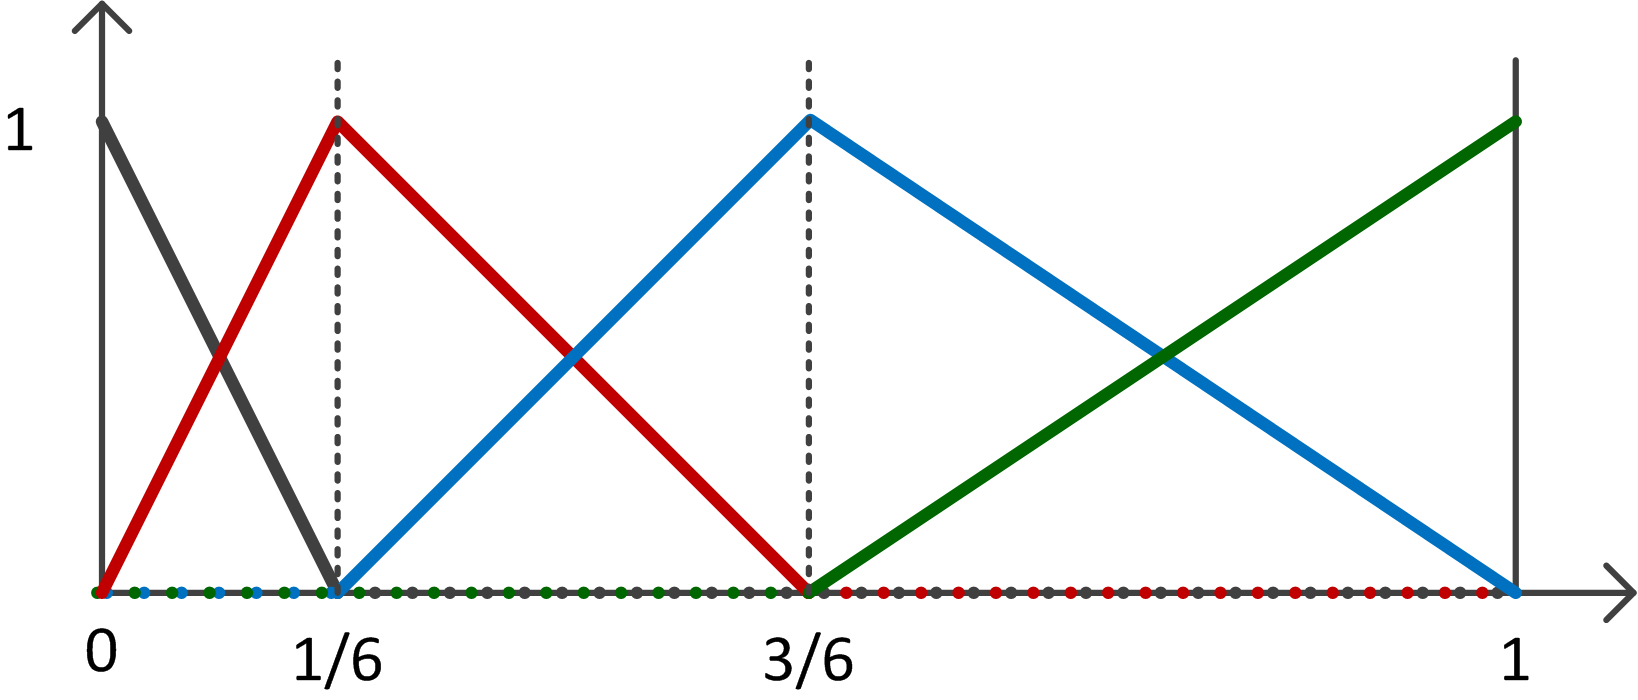
\includegraphics[width=9cm]{Content/Numerik/FEMHand}
\end{minipage}\\

$R^n\cdot a +r^n=0 \qquad\Rightarrow\qquad
\begin{bmatrix}
	-6 & 6 & 0 & 0\\
	6 & -9 & 3 & 0\\
	0 & 3 & -5 & 2\\
	0 & 0 & 2 & -2\\
\end{bmatrix}\cdot
\begin{bmatrix}
	10\\
	a_1\\
	a_2\\
	20
\end{bmatrix}+
\begin{bmatrix}
	5/3\\
	5\\
	25/3\\
	5
\end{bmatrix}=
\begin{bmatrix}
	0\\
	0\\
	0\\
	0
\end{bmatrix}\qquad\Rightarrow\qquad
\begin{bmatrix}
	6 & -9 & 3 & 0\\
	0 & 3 & -5 & 2\\
\end{bmatrix}\cdot
\begin{bmatrix}
	10\\
	a_1\\
	a_2\\
	20
\end{bmatrix}+
\begin{bmatrix}
	5/3\\
	5\\
	25/3\\
	5
\end{bmatrix}=
\begin{bmatrix}
	0\\
	0\\
	0\\
	0
\end{bmatrix}	
$\\
\\

$\qquad\Rightarrow\qquad
\begin{bmatrix}
	-9 & 3\\
	3 & -5\\
\end{bmatrix}\cdot
\begin{bmatrix}
	a_1\\
	a_2\\
\end{bmatrix}+
\begin{bmatrix}
	6\cdot 10\\
	2\cdot 20\\
\end{bmatrix}+
\begin{bmatrix}
	5\\
	25/3\\
\end{bmatrix}
=0\qquad\Rightarrow\qquad
\begin{bmatrix}
	-9 & 3\\
	3 & -5\\
\end{bmatrix}\cdot
\begin{bmatrix}
	a_1\\
	a_2\\
\end{bmatrix}=
\begin{bmatrix}
	-65\\
	-145/3\\
\end{bmatrix}\qquad\Rightarrow\qquad
\begin{bmatrix}
	a_1\\
	a_2\\
\end{bmatrix}=
\begin{bmatrix}
	235/18\\
	35/2\\
\end{bmatrix}
$\\
\\
$
\qquad\Rightarrow\qquad \tilde{u}(x)=10\cdot v_0(x)+\frac{235}{18} v_1(x)+\frac{35}{2}\cdot v_2(x)+20\cdot v_3(x)=
$




\subsubsection{h-Strategie}

Die Grundidee der h-Strategie ist die Verfeinerung der Auflösung. Mit anderen Worten die Maschenbreite $h$ wird verkleinert. Um den ganzen Bereich dennoch abdecken zu können sind mehr Maschen notwendig.

\subsubsection{p-Strategie}
Bei der p-Strategie bleibt das Netz bestehen. Die Ansatzfunktionen sollen nun durch Polynome höherer Ordnung zusammengesetzt werden, dazu werden neue Knoten und Knotenvariablen eingeführt werden.\\

\textbf{Problemstellung:} $u''(x)+f(x)=0\qquad u(0)=a_0\qquad u(1)=a_6$\\

Die Approximation soll auf dem gleichverteilten Intervallen gelten: $[0,1/3]$,\quad $[1/3,2/3]$,\quad $[2/3,1]$\\

\begin{minipage}{4cm}
	Formfunktionen:\\

	$q_1(x)=(1-x)\cdot(1-2x)$\\
	$q_2(x)=4x\cdot(1-x)$\\
	$q_3(x)=-x\cdot(1-2x)$\\
	
	Elementmatrize: $\boxed{E=\frac{1}{3}
	\begin{bmatrix}
		-7& 8 & -1\\
		8& -16& 8\\
		-1& 8& -7	
	\end{bmatrix}}$\\
\end{minipage}
\hfill
\begin{minipage}{8cm}
	\begin{tabular}{lc|c|c}
		$x\in$&$[0,1/3]$&$[1/3,2/3]$&$[2/3,1]$\\
		\hline
		$v_0=$&$q_1(3x)$&$0$&$0$\\
		$v_1=$&$q_2(3x)$&$0$&$0$\\
		$v_2=$&$q_3(3x)$&$q_1(3x-1)$&$0$\\
		$v_3=$&$0$&$q_2(3x-1)$&$0$\\
		$v_4=$&$0$&$q_3(3x-1)$&$q_1(3x-2)$\\
		$v_5=$&$0$&$0$&$q_2(3x-2)$\\
		$v_6=$&$0$&$0$&$q_3(3x-2)$\\
	\end{tabular}
\end{minipage}
\hfill
\begin{minipage}{6cm}
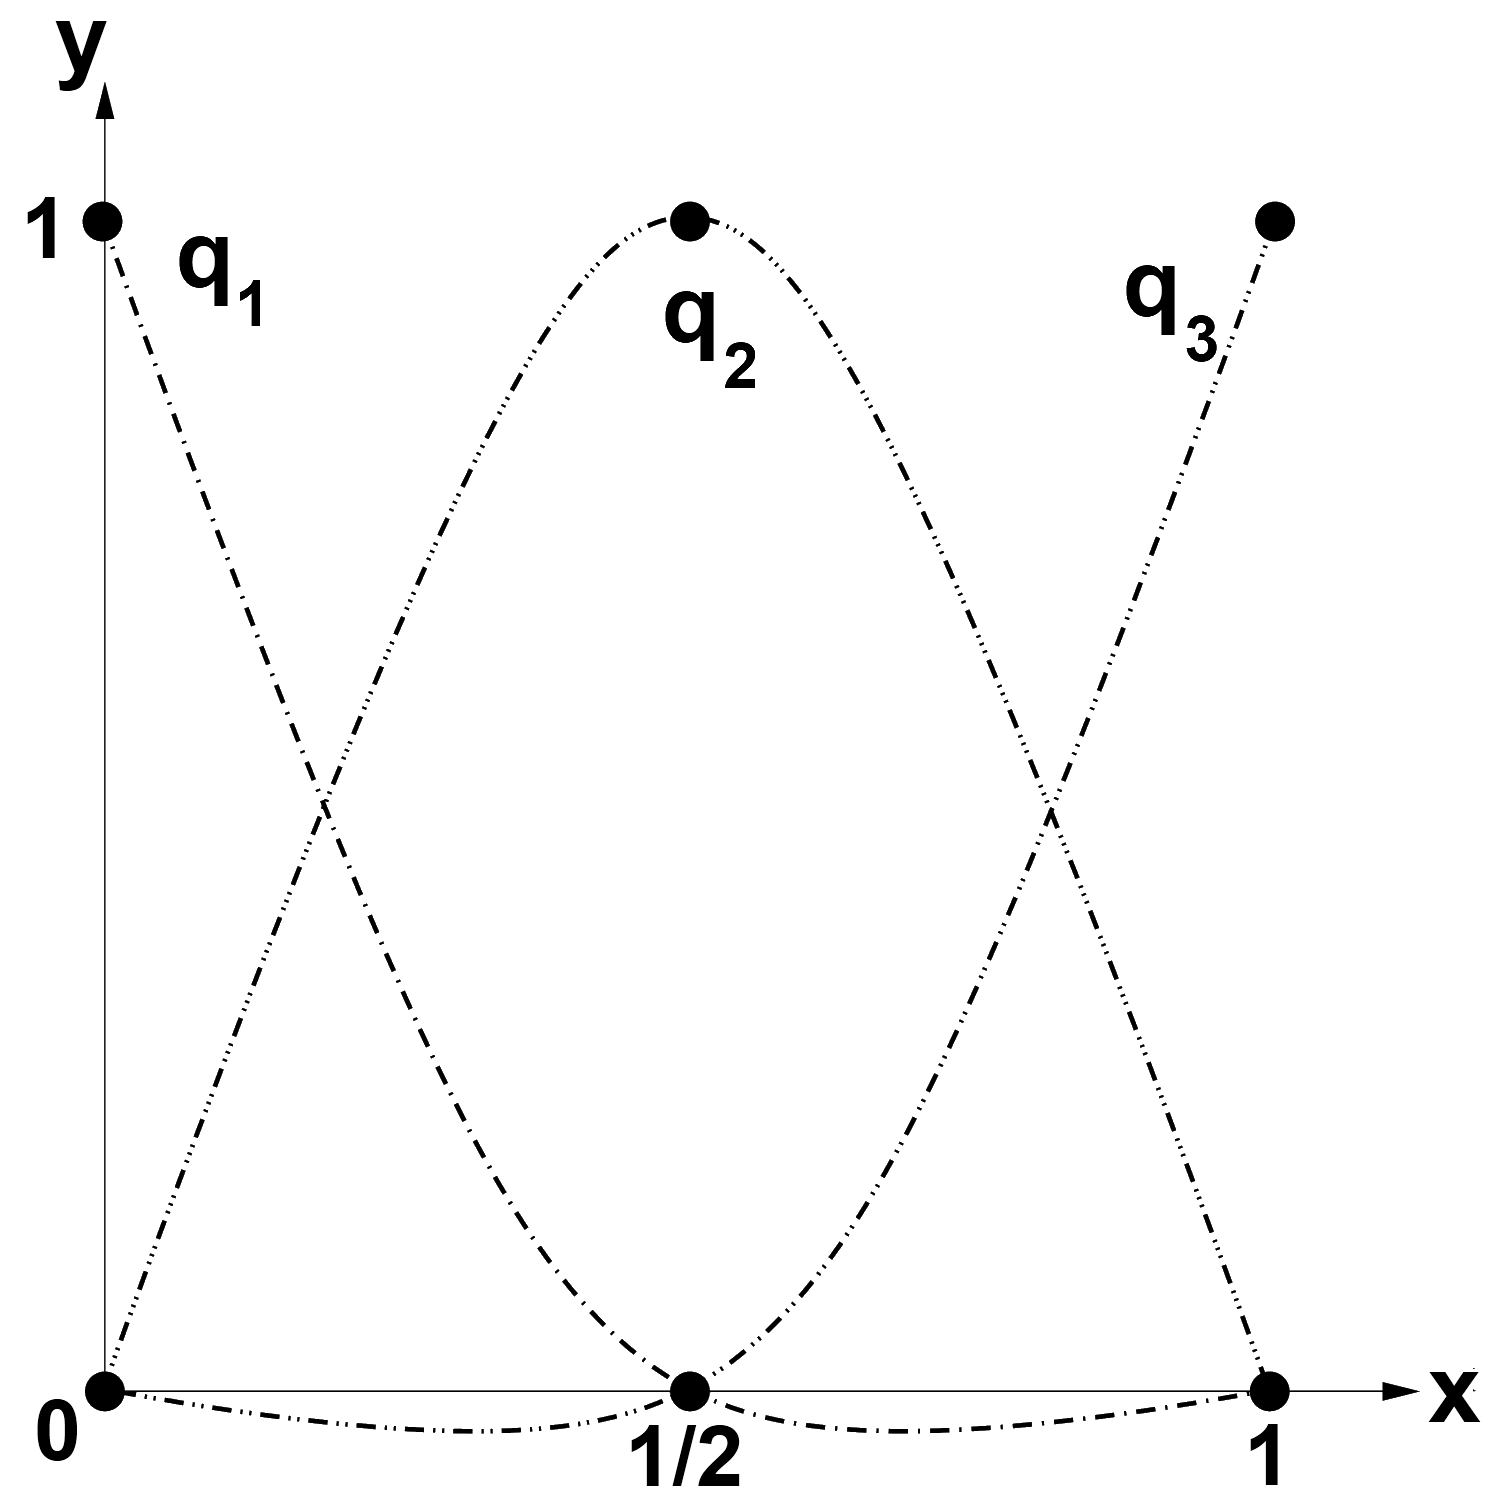
\includegraphics[width=6cm]{Content/Numerik/FEM2Ord}
\end{minipage}\\

$\underset{\text{Ritzsche Matrize $R^{(8)}$ für } h=1/3}{\underbrace{\begin{bmatrix}
	-7& 8 & -1& 0& 0& 0& 0\\
	 8& -16& 8& 0& 0& 0& 0\\
	-1& 8& -14& 8& -1& 0& 0\\ 
	 0& 0& 8& -16& 8& 0& 0\\
	 0& 0& -1& 8& -14& 8& -1\\ 
	 0& 0& 0& 0& 8& -16& 8\\
	 0& 0& 0& 0& -1& 8& -7	
\end{bmatrix}}}\cdot\begin{bmatrix}
	a_0\\
	a_1\\
	a_2\\
	a_3\\
	a_4\\
	a_5\\
	a_6\\
\end{bmatrix}
+\underset{\text{Ritzscher Vektor $r^{(8)}$ für } h=1/3}{\underbrace{\begin{bmatrix}
	\int\limits_{0}^{1}{f(x)\cdot v_0(x)dx}\\
	\int\limits_{0}^{1}{f(x)\cdot v_1(x)dx}\\
	\int\limits_{0}^{1}{f(x)\cdot v_2(x)dx}\\
	\int\limits_{0}^{1}{f(x)\cdot v_3(x)dx}\\
	\int\limits_{0}^{1}{f(x)\cdot v_4(x)dx}\\
	\int\limits_{0}^{1}{f(x)\cdot v_5(x)dx}\\
	\int\limits_{0}^{1}{f(x)\cdot v_6(x)dx}\\
\end{bmatrix}}}=
\begin{bmatrix}
	0\\
	0\\
	0\\
	0\\
	0\\
	0\\
	0\\
	0\\
\end{bmatrix}
$\\

\textbf{Vorteil der p-Strategie gegenüber der h-Strategie:} Bei beiden Strategien steigt die Dimension der Systemmatrizen an. Es besteht jedoch die berechtigte Hoffnung, dass der Zuwachs der benötigt wird, um eine vergleichbare Genauigkeit zu errreichen, bei der p-Strategie weitaus geringer ist als bei der h-Strategie. 

\subsection{Konformität und Vollständigkeit}
Muss nun die Approximationslösung zweimal ableitbar sein, so gilt der Ansatz des letzten Abschnitt nicht mehr als konform.

Um die einmalige Differenzierbarkeit an den Knoten zu gewährleisten müssen neue Grundfunktionen gefunden werden.\\

$\tilde{u}(x)=a_0v_0(x)+a_1v_1(x)+a_2v_2(x)+a_3v_3(x)+\tilde{a}_0\tilde{v}_0(x)+\tilde{a}_1\tilde{v}_1(x)+\tilde{a}_2\tilde{v}_2(x)+\tilde{a}_3\tilde{v}_3(x)$\\

Zwei Grundfunktionen stellen den richtigen Wert and den Knoten sicher. Zwei weitere Grundfunktionen werden benötigt um die erste Ableitung (Steigung) an den Übergangknoten sicherzustellen, sie sorgen für die Vollständigkeit der Grundfunktionen. (Ohne die zwei weiteren Grundfunktionen wäre an den Übergangsknoten nur eine Steigung von Null möglich.)

\subsection{Hermetische Polynome dritter Ordnung}
Übereinstimmung bis zur 1.Ableitung an den Knotenpunkten\\

\textbf{Problemstellung:} $u''(x)+f(x)=0\qquad u(0)=a_0\qquad u'(0)=\tilde{a}_0 \qquad u(1)=a_3\qquad  u'(1)=\tilde{a}_3$\\

Die Approximation soll auf dem gleichverteilten Intervallen gelten: $[0,1/3]$,\quad $[1/3,2/3]$,\quad $[2/3,1]$\\

\begin{minipage}{4cm}
Formfunktionen:\\
$h_1(x)=2x^3-3x^2+1$\\
$h_2(x)=x^3-2x^2+x$\\
$h_3(x)=-2x^3+3x^2$\\
$h_4(x)=x^3-x^2$
\end{minipage}
\hfill
\begin{minipage}{8cm}
	\begin{tabular}{lc|c|c}
		$x\in$&$[0,1/3]$&$[1/3,2/3]$&$[2/3,1]$\\
		\hline
		$v_0=$&$h_1(3x)$&$0$&$0$\\
		$\tilde{v}_0=$&$\frac 13 h_2(3x)$&$0$&$0$\\
		$v_1=$&$h_3(3x)$&$h_1(3x-1)$&$0$\\
		$\tilde{v}_1=$&$\frac 13 h_4(3x)$&$\frac 13 h_2(3x-1)$&$0$\\
		$v_2=$&$0$&$h_3(3x-1)$&$h_1(3x-2)$\\
		$\tilde{v}_2=$&$0$&$\frac 13 h_4(3x-1)$&$\frac 13 h_2(3x-2)$\\
		$v_3=$&$0$&$0$&$h_3(3x-2)$\\
		$\tilde{v}_3=$&$0$&$0$&$\frac 13 h_2(3x-1)$\\
	\end{tabular}
\end{minipage}
\hfill
\begin{minipage}{6cm}
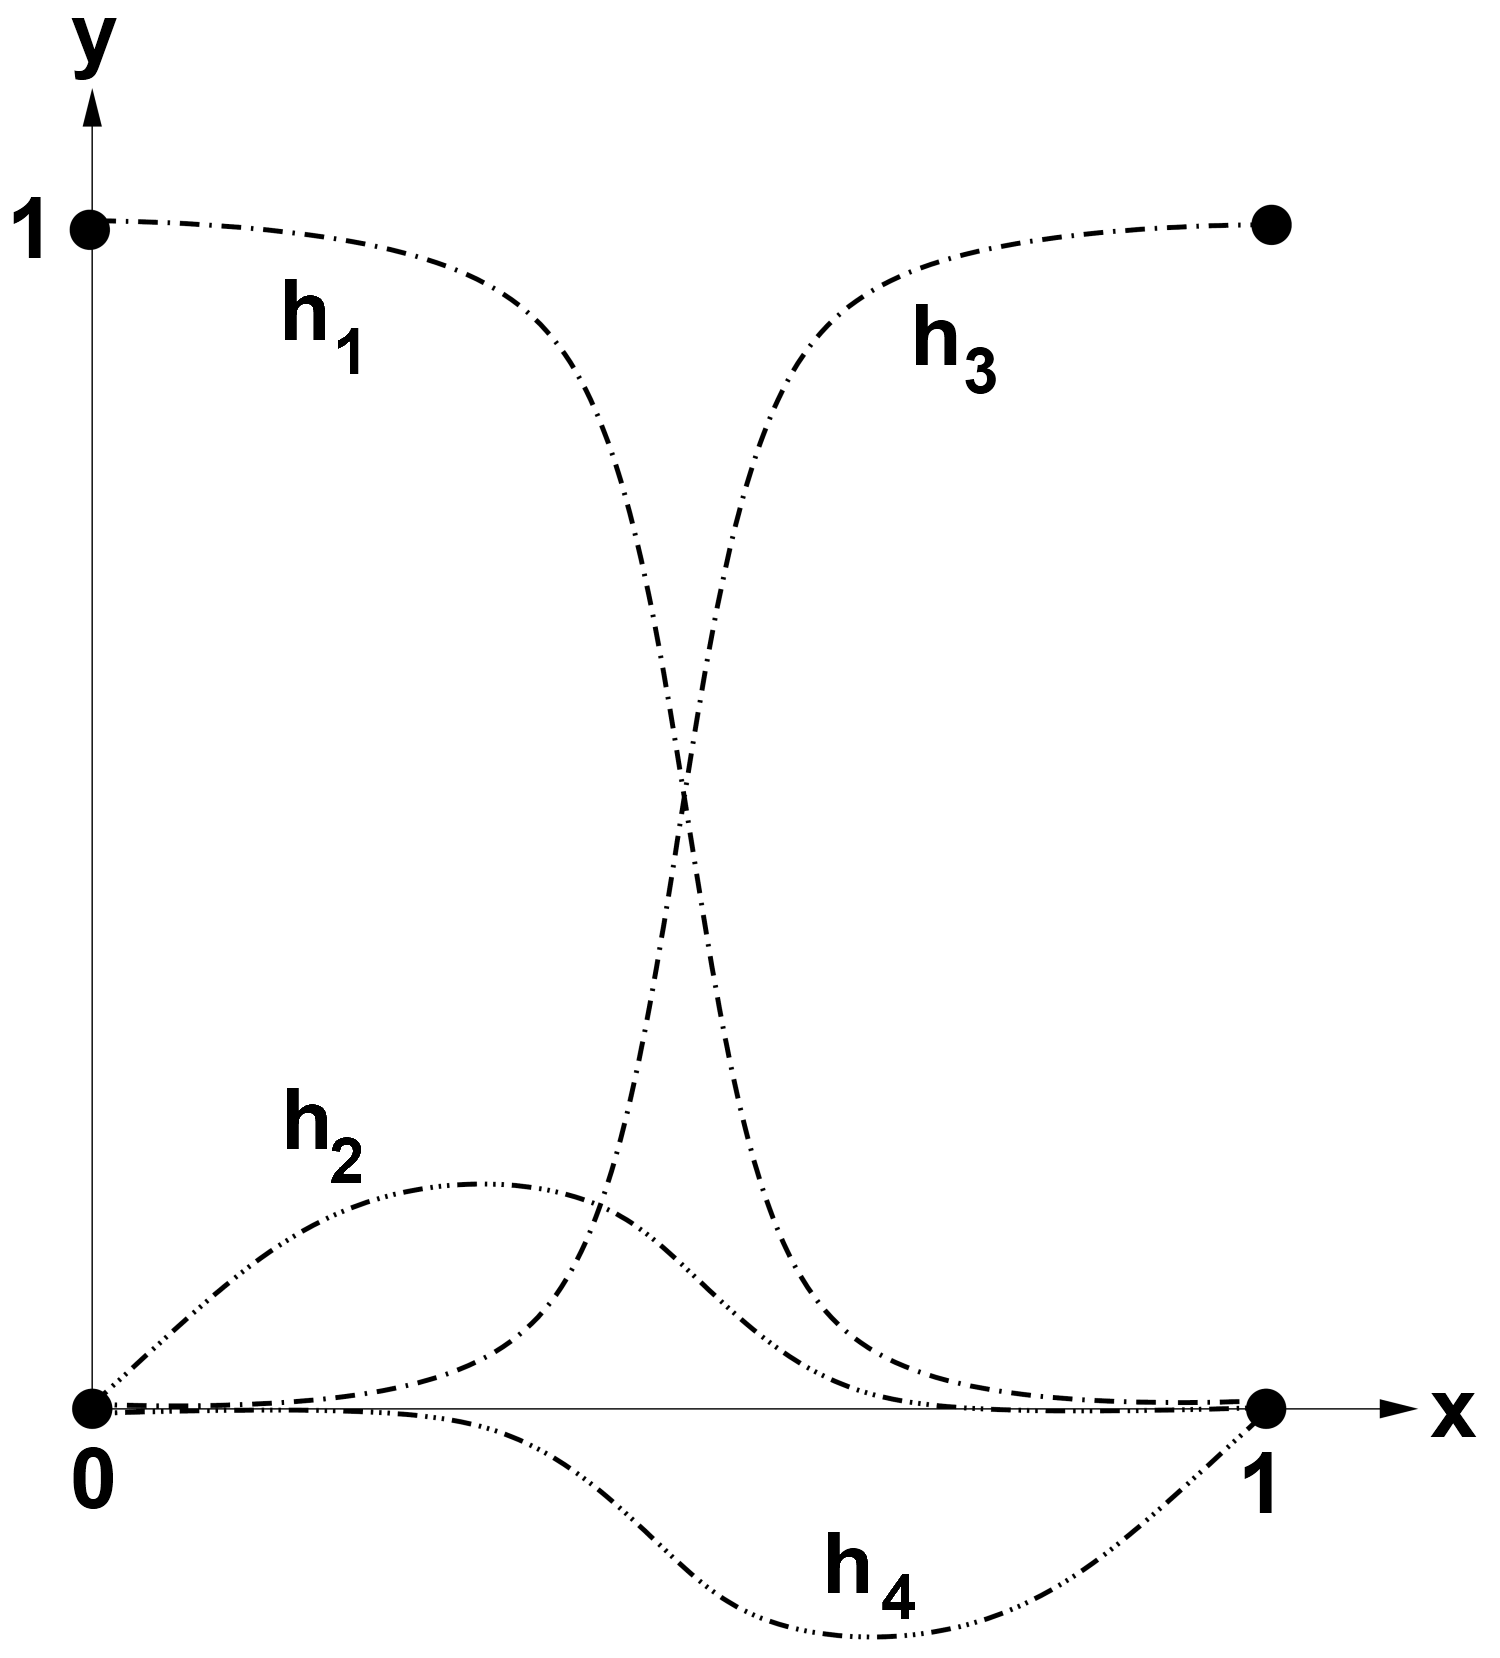
\includegraphics[width=6cm]{Content/Numerik/FEM3Ord}
\end{minipage}\\
$E=\frac{1}{30}
\begin{bmatrix}
	-36 & -3 & 36 & -3\\
	-3 & -4 & 3 & 1\\
	36 & 3 & -36 & 3\\
	-3 & 1 & 3 & -4\\
\end{bmatrix}\qquad\Rightarrow\qquad
\boxed{M=\frac{1}{30\cdot h}
\begin{bmatrix}
	-36 & -3\cdot h & 36 & -3\cdot h\\
	-3\cdot h & -4\cdot h^2 & 3\cdot h & 1\cdot h^2\\
	36 & 3\cdot h & -36 & 3\cdot h\\
	-3\cdot h & 1\cdot h^2 & 3\cdot h & -4\cdot h^2\\
\end{bmatrix}}$\\
\\


$\underset{\text{Ritzsche Matrize $R^{(8)}$ für } h=1/3}{\underbrace{\frac{3}{30}\begin{bmatrix}
	-36 & -1 & 36 & -1 & 0  & 0  & 0  & 0 \\
	-1  & -4/9  & 1  & 1/9  & 0  & 0  & 0  & 0\\
	36  & 1  & -72  & 0  & 36  & -1  & 0  & 0\\
	-1  & 1/9  & 0  & -8/9  & 1  & 1/9  & 0  & 0\\
	0  & 0  & 36  & 1  & -72  & 0  & 36  & -1\\
	0  & 0  & -1  & 1/9  & 0  & -8/9  & 1  & 1/9\\
	0  & 0  & 0  & 0  & 36  & 1  & -36  & 1\\
	0  & 0  & 0  & 0  & -1  & 1/9  & 1  & -4/9\\
\end{bmatrix}}}\cdot\begin{bmatrix}
	a_0\\
	\tilde{a}_0\\
	a_1\\
	\tilde{a}_1\\
	a_2\\
	\tilde{a}_2\\
	a_3\\
	\tilde{a}_3\\
\end{bmatrix}
+\underset{\text{Ritzscher Vektor $r^{(8)}$ für } h=1/3}{\underbrace{\begin{bmatrix}
	\int\limits_{0}^{1}{f(x)\cdot v_0(x)dx}\\
	\int\limits_{0}^{1}{f(x)\cdot \tilde{v}_0(x)dx}\\
	\int\limits_{0}^{1}{f(x)\cdot v_1(x)dx}\\
	\int\limits_{0}^{1}{f(x)\cdot \tilde{v}_1(x)dx}\\
	\int\limits_{0}^{1}{f(x)\cdot v_2(x)dx}\\
	\int\limits_{0}^{1}{f(x)\cdot \tilde{v}_2(x)dx}\\
	\int\limits_{0}^{1}{f(x)\cdot v_3(x)dx}\\
	\int\limits_{0}^{1}{f(x)\cdot \tilde{v}_3(x)dx}\\
\end{bmatrix}}}=
\begin{bmatrix}
	0\\
	0\\
	0\\
	0\\
	0\\
	0\\
	0\\
	0\\
\end{bmatrix}
$\\







%\subsection{FEM für parabolische PDEs}